\section{Use case scenarios}
\label{section:Use case scenarios}

Once the scene is rendered in 3D, it enables free viewpoint. Using this kind of technology for meeting rooms is what Logitech is interested in. Finding an appropriate point of view is an interesting and complex problem. This chapter proposes two meeting room use case scenarios and an alternative one:

\begin{enumerate}
    \item Positioning the camera regarding the head pose
    \item Multiple persons: positioning the camera regarding the speaker
    \item Streaming for gamer
\end{enumerate}

\subsection{How to set the pose of a camera in a 3D space?}

To set the camera pose in 3D environments, the extrinsic camera matrix is used. This matrix describes the location of the camera in the world and what direction it is pointing. It is composed of two elements: a 3x3 rotation matrix $\mathbf{R}$ and a 3x1 translation vector $\mathbf{t}$, see equation (\ref{equation:extrinsic_camera_matrix}).

\begin{equation}
    [R | \boldsymbol{t}]=\left[\begin{array}{lll|l}
    {r_{1,1}} & {r_{1,2}} & {r_{1,3}} & {t_{1}} \\
    {r_{2,1}} & {r_{2,2}} & {r_{2,3}} & {t_{2}} \\
    {r_{3,1}} & {r_{3,2}} & {r_{3,3}} & {t_{3}}
    \end{array}\right]
    \label{equation:extrinsic_camera_matrix}
\end{equation}

Determining this matrix is not intuitive. The "Look-At" approach describes in \cite{noauthor_dissecting_nodate} and proposes by OpenGL \cite{noauthor_glulookat_nodate} is probably the more natural way. It needs three information to determine and compute the extrinsic matrix. These are the camera's position $\mathbf{C}$ in the world coordinate system, what the camera is looking at $\mathbf{p}$ and the "up" direction $\mathbf{u}$. The algorithm to compute the rotation matrix is the following:

\begin{enumerate}
    \item Compute $\mathbf{L} = \mathbf{p} - \mathbf{C}$
    \item Normalise $\mathbf{L}$
    \item Compute $\mathbf{s}=\mathbf{L} \times \mathbf{u}$
    \item Normalise $\mathbf{s}$
    \item Compute $\mathbf{u^{\prime}} = \mathbf{s} \times \mathbf{L}$
\end{enumerate}

\begin{equation}
    \mathbf{R}=\left[\begin{array}{ccc}{s_{1}} & {s_{2}} & {s_{3}} \\ {u_{1}^{\prime}} & {u_{2}^{\prime}} & {u_{3}^{\prime}} \\ {-L_{1}} & {-L_{2}} & {-L_{3}}\end{array}\right]
    \label{equation:look-at}
\end{equation}

The translation vector is then calculated as follow:

\begin{equation}
    \mathbf{t}=-\mathbf{R C}
\end{equation}


\subsection{Positioning the camera regarding the head pose}

Often 2D RGB cameras are not placed directly in front of the speaker in a video conference situation which could be disturbing to interact with the interlocutor. Placing the virtual camera in front of the head/gaze is a proposed approach to improve the immersion. Doing it automatically is the idea. For this purpose, the head/gaze pose has to be determined. \textit{PifPaf} \cite{kreiss_pifpaf_2019}, which is a 2D human pose estimation framework, is used to estimate the head/gaze pose. It detects keypoints in a human body. Three keypoints detected by \textit{PifPaf} are used to determine where to put the camera. These three keypoints are the following: right eye, left eye, nose. They are detected in the 2D RGB images. Thanks to the synchronised captures depth image, a 3D transformation of these keypoints is calculated by using equation (\ref{equation:2dTO3d}). Then 3D geometrical calculations are done to determine where to put the virtual camera in the 3D space. The origin of the 3D vectors is placed on the 3D nose keypoint, see figure \ref{figure:head_vectors}.

\begin{figure}[H]
    \centering
    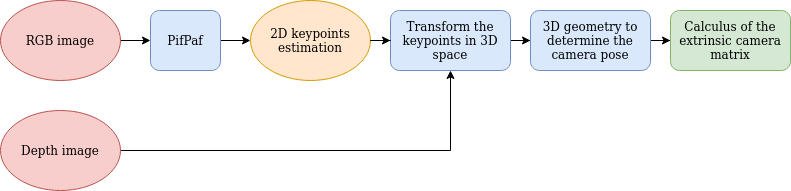
\includegraphics[width=0.85\textwidth]{images/scenario/pipeline_pifpaf.png}
    \caption{Proposed pipeline for 3D virtual camera pose determination. Input: red boxes. Output: green box.}
    \label{figure:pipeline_pifpaf}
\end{figure}

These are the steps of the 3D geometrical calculations, see also figure :

\begin{enumerate}
    \item Compute $ \mathbf{R}=\mathbf{Y} \times \mathbf{P}$
    \item Normalise $\mathbf{R}$
    \item Compute $\mathbf{G}=-(\mathbf{P}+\mathbf{Y})$
    \item Normalise $\mathbf{G}$
    \item Compute $\mathbf{B}=\mathbf{R}+\mathbf{G}$
    \item Normalise $\mathbf{B}\rightarrow$ Camera pose
\end{enumerate}

\begin{figure}[H]
    \centering
    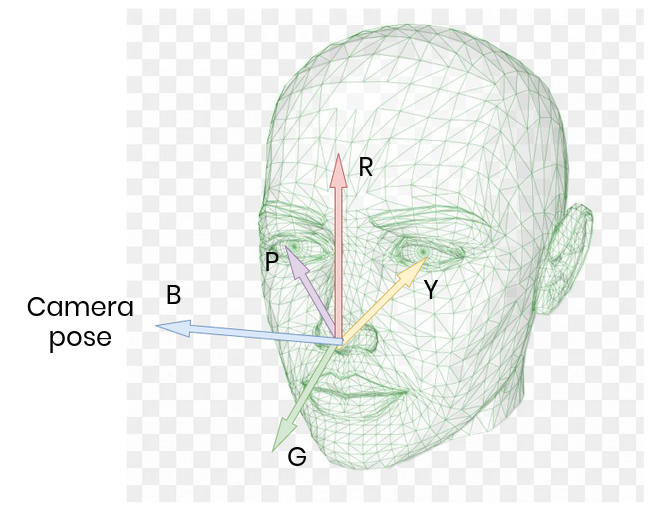
\includegraphics[width=0.45\textwidth]{images/scenario/head_vectors.png}
    \caption{Sketch of the 3D created vectors}
    \label{figure:head_vectors}
\end{figure}

$\mathbf{C}$ position is determined as the end of the 3D blue vectors. 3D nose keypoint is determined as the look at point ${\mathbf{p}}$. $\mathbf{u}$ is defined as $[0,-1,0]$. Then the extrinsic camera matrix is computed as explained in the previous section.

\subsubsection{Result}

Figure \ref{figure:00265_head_vector} shows a selected frame where the calculated vectors have been drawn. Because the position of the vectors is changing for each frame, it results in a flickering effect in the camera movement. To avoid this effect, a simple moving median filter is applied.

\begin{figure}[H]
    \centering
    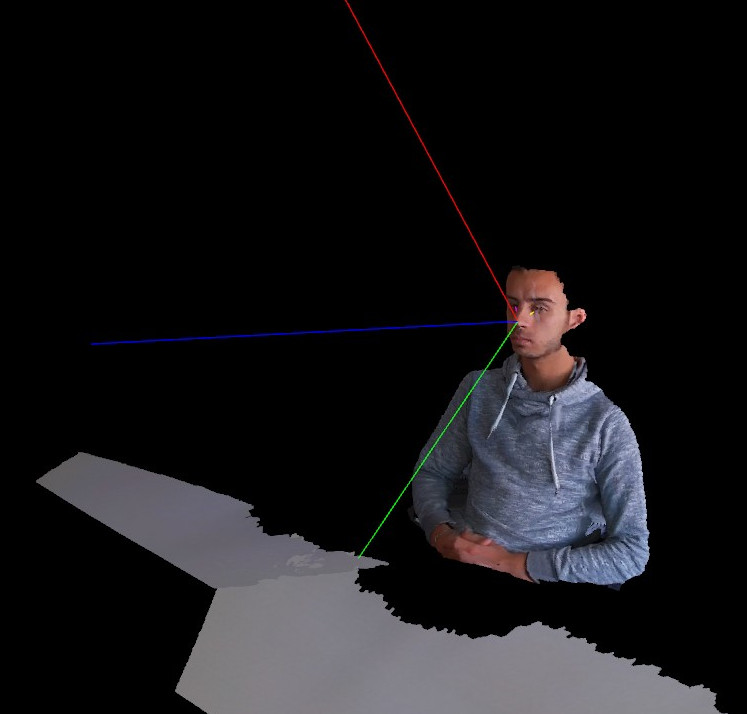
\includegraphics[width=0.45\textwidth]{images/scenario/00265_head_vector.jpg}
    \caption{3D vectors in a selected frame}
    \label{figure:00265_head_vector}
\end{figure}

Figure \ref{figure:diff_head_pose} shows frames with different viewpoints. $\mathbf{C}$ corresponds to the end of the blue vector. The look at point $\mathbf{p}$ corresponds to the 3D nose keypoint coordinate.

\begin{figure}[H]
\centering
  \begin{subfigure}[b]{0.32 \textwidth}
    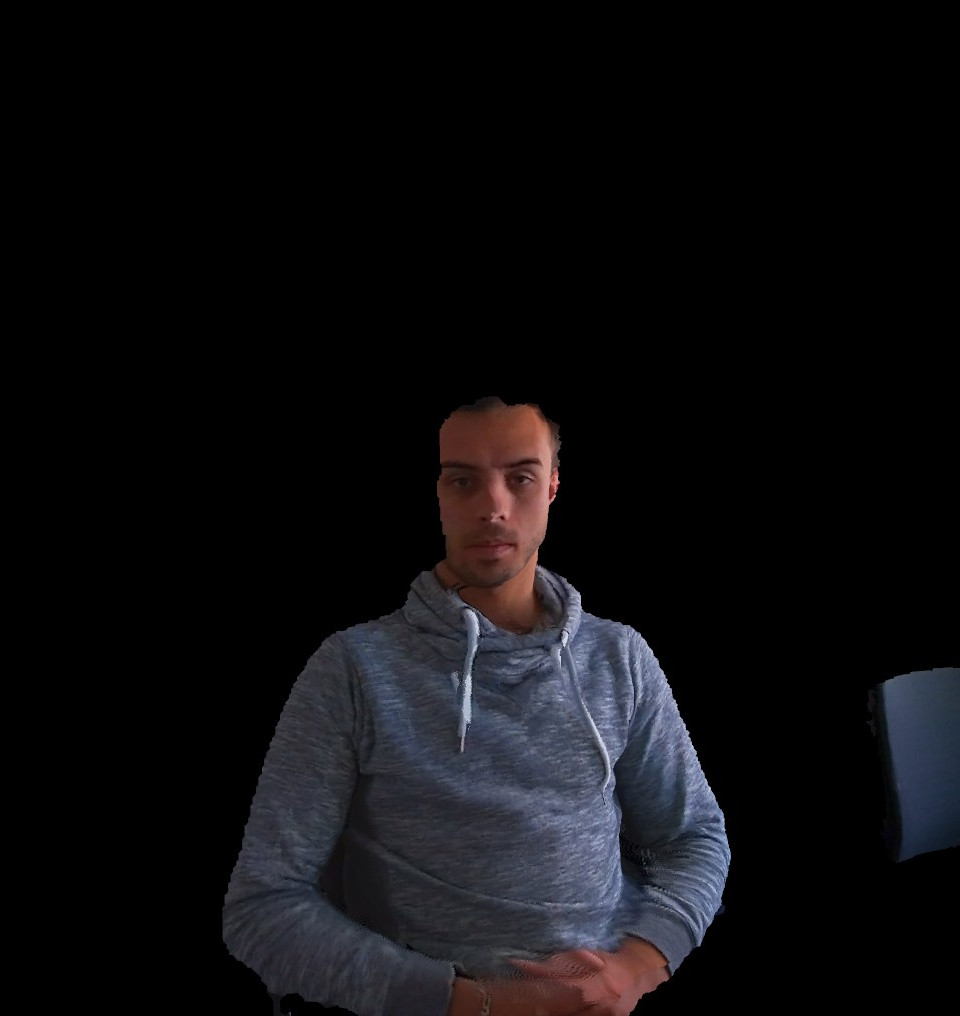
\includegraphics[width=\textwidth]{images/scenario/00465_head.jpg}
    \caption{Head pose point of view 1}
    \label{figure:00465_head}
  \end{subfigure}
  \hfill
  \begin{subfigure}[b]{0.32 \textwidth}
    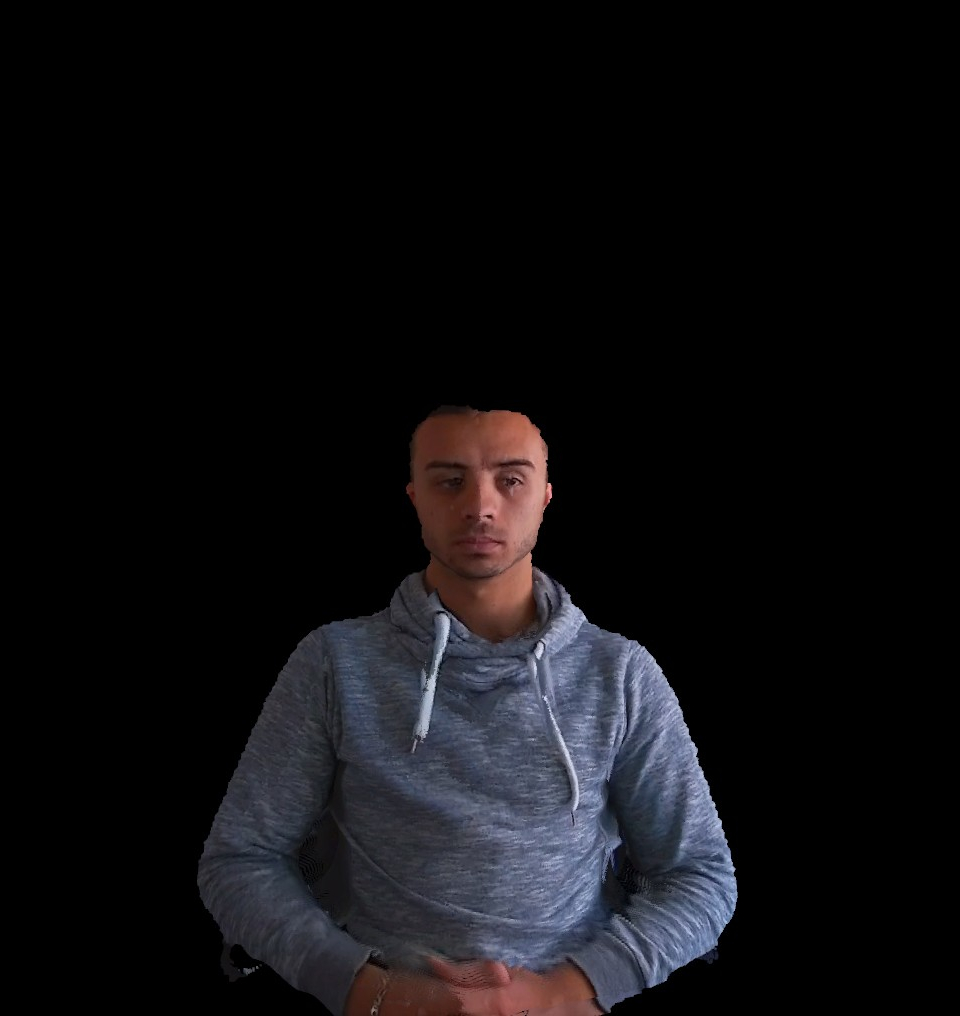
\includegraphics[width=\textwidth]{images/scenario/00267_head.jpg}
    \caption{Head pose point of view 2}
    \label{figure:00267_head}
  \end{subfigure}
  \hfill
  \begin{subfigure}[b]{0.32 \textwidth}
    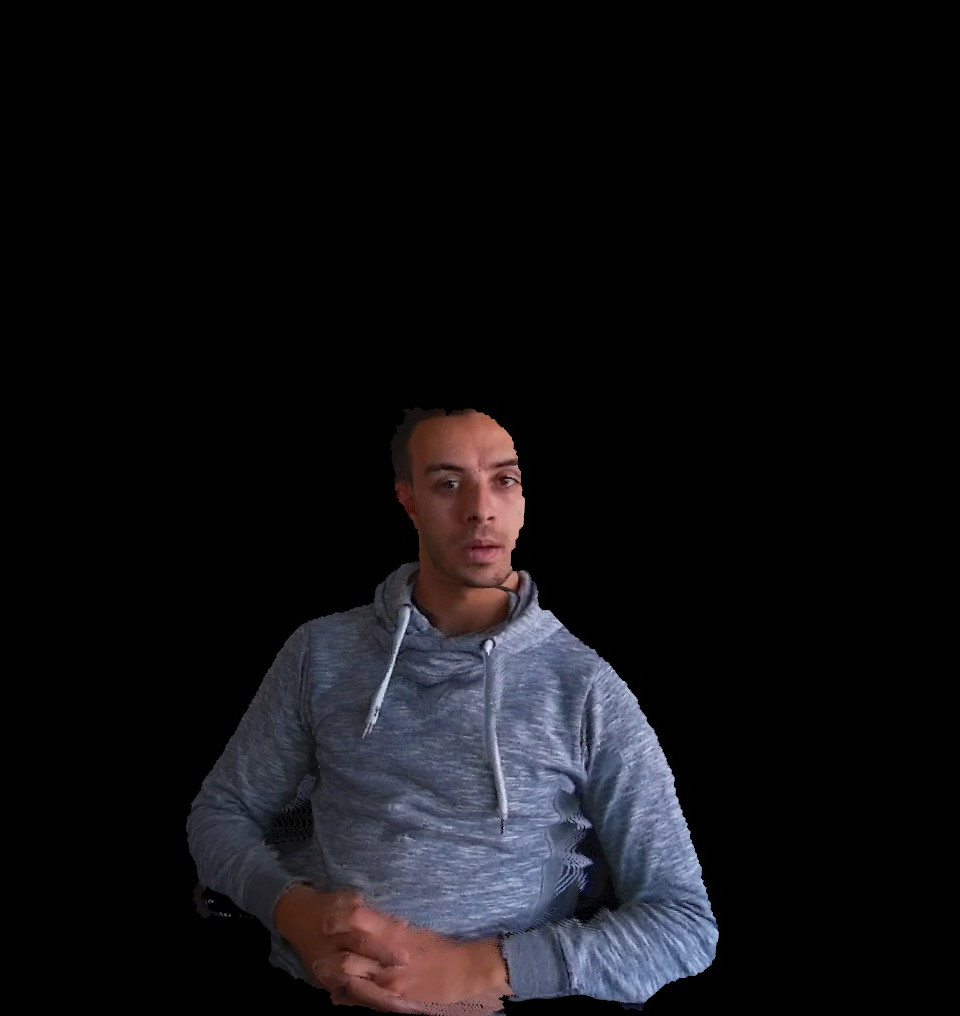
\includegraphics[width=\textwidth]{images/scenario/00620_head.jpg}
    \caption{Head pose point of view 3}
    \label{figure:00620_head}
  \end{subfigure}
  \caption{Different viewpoint based on the head/gaze pose approach}
  \label{figure:diff_head_pose}
\end{figure}


\subsubsection{Discussion}

Using a head/gaze pose estimation to place the camera in the 3D world space increases the immersion. However, deeper work should be done in order to avoid disturbing movement of the camera. The median moving filter is not sufficient.



\subsection{Multiple persons: positioning the camera regarding the speaker}

 In case of multiple persons in a conference room,  everyone can't be well placed regarding a 2D RGB camera.  Therefore, people attending the discussion by their own computer could feel put apart of it. Moving manually the camera is not really an option. The 3D rendering of the scene enables to move virtually the camera pose in order to face always the speakers in the room. Figure \ref{figure:two_persons_virtualview} shows the two original 2D views and the virtual view created thanks to the 3D rendering of the scene. Only two cameras have been used for the rendering. Increasing the number of cameras would have given a better reconstruction. Indeed, when data of the people are missing, the wall behind is visible instead, see figure \ref{figure:00790_background}.
 
 \begin{figure}[H]
\centering
  \begin{subfigure}[b]{0.48 \textwidth}
    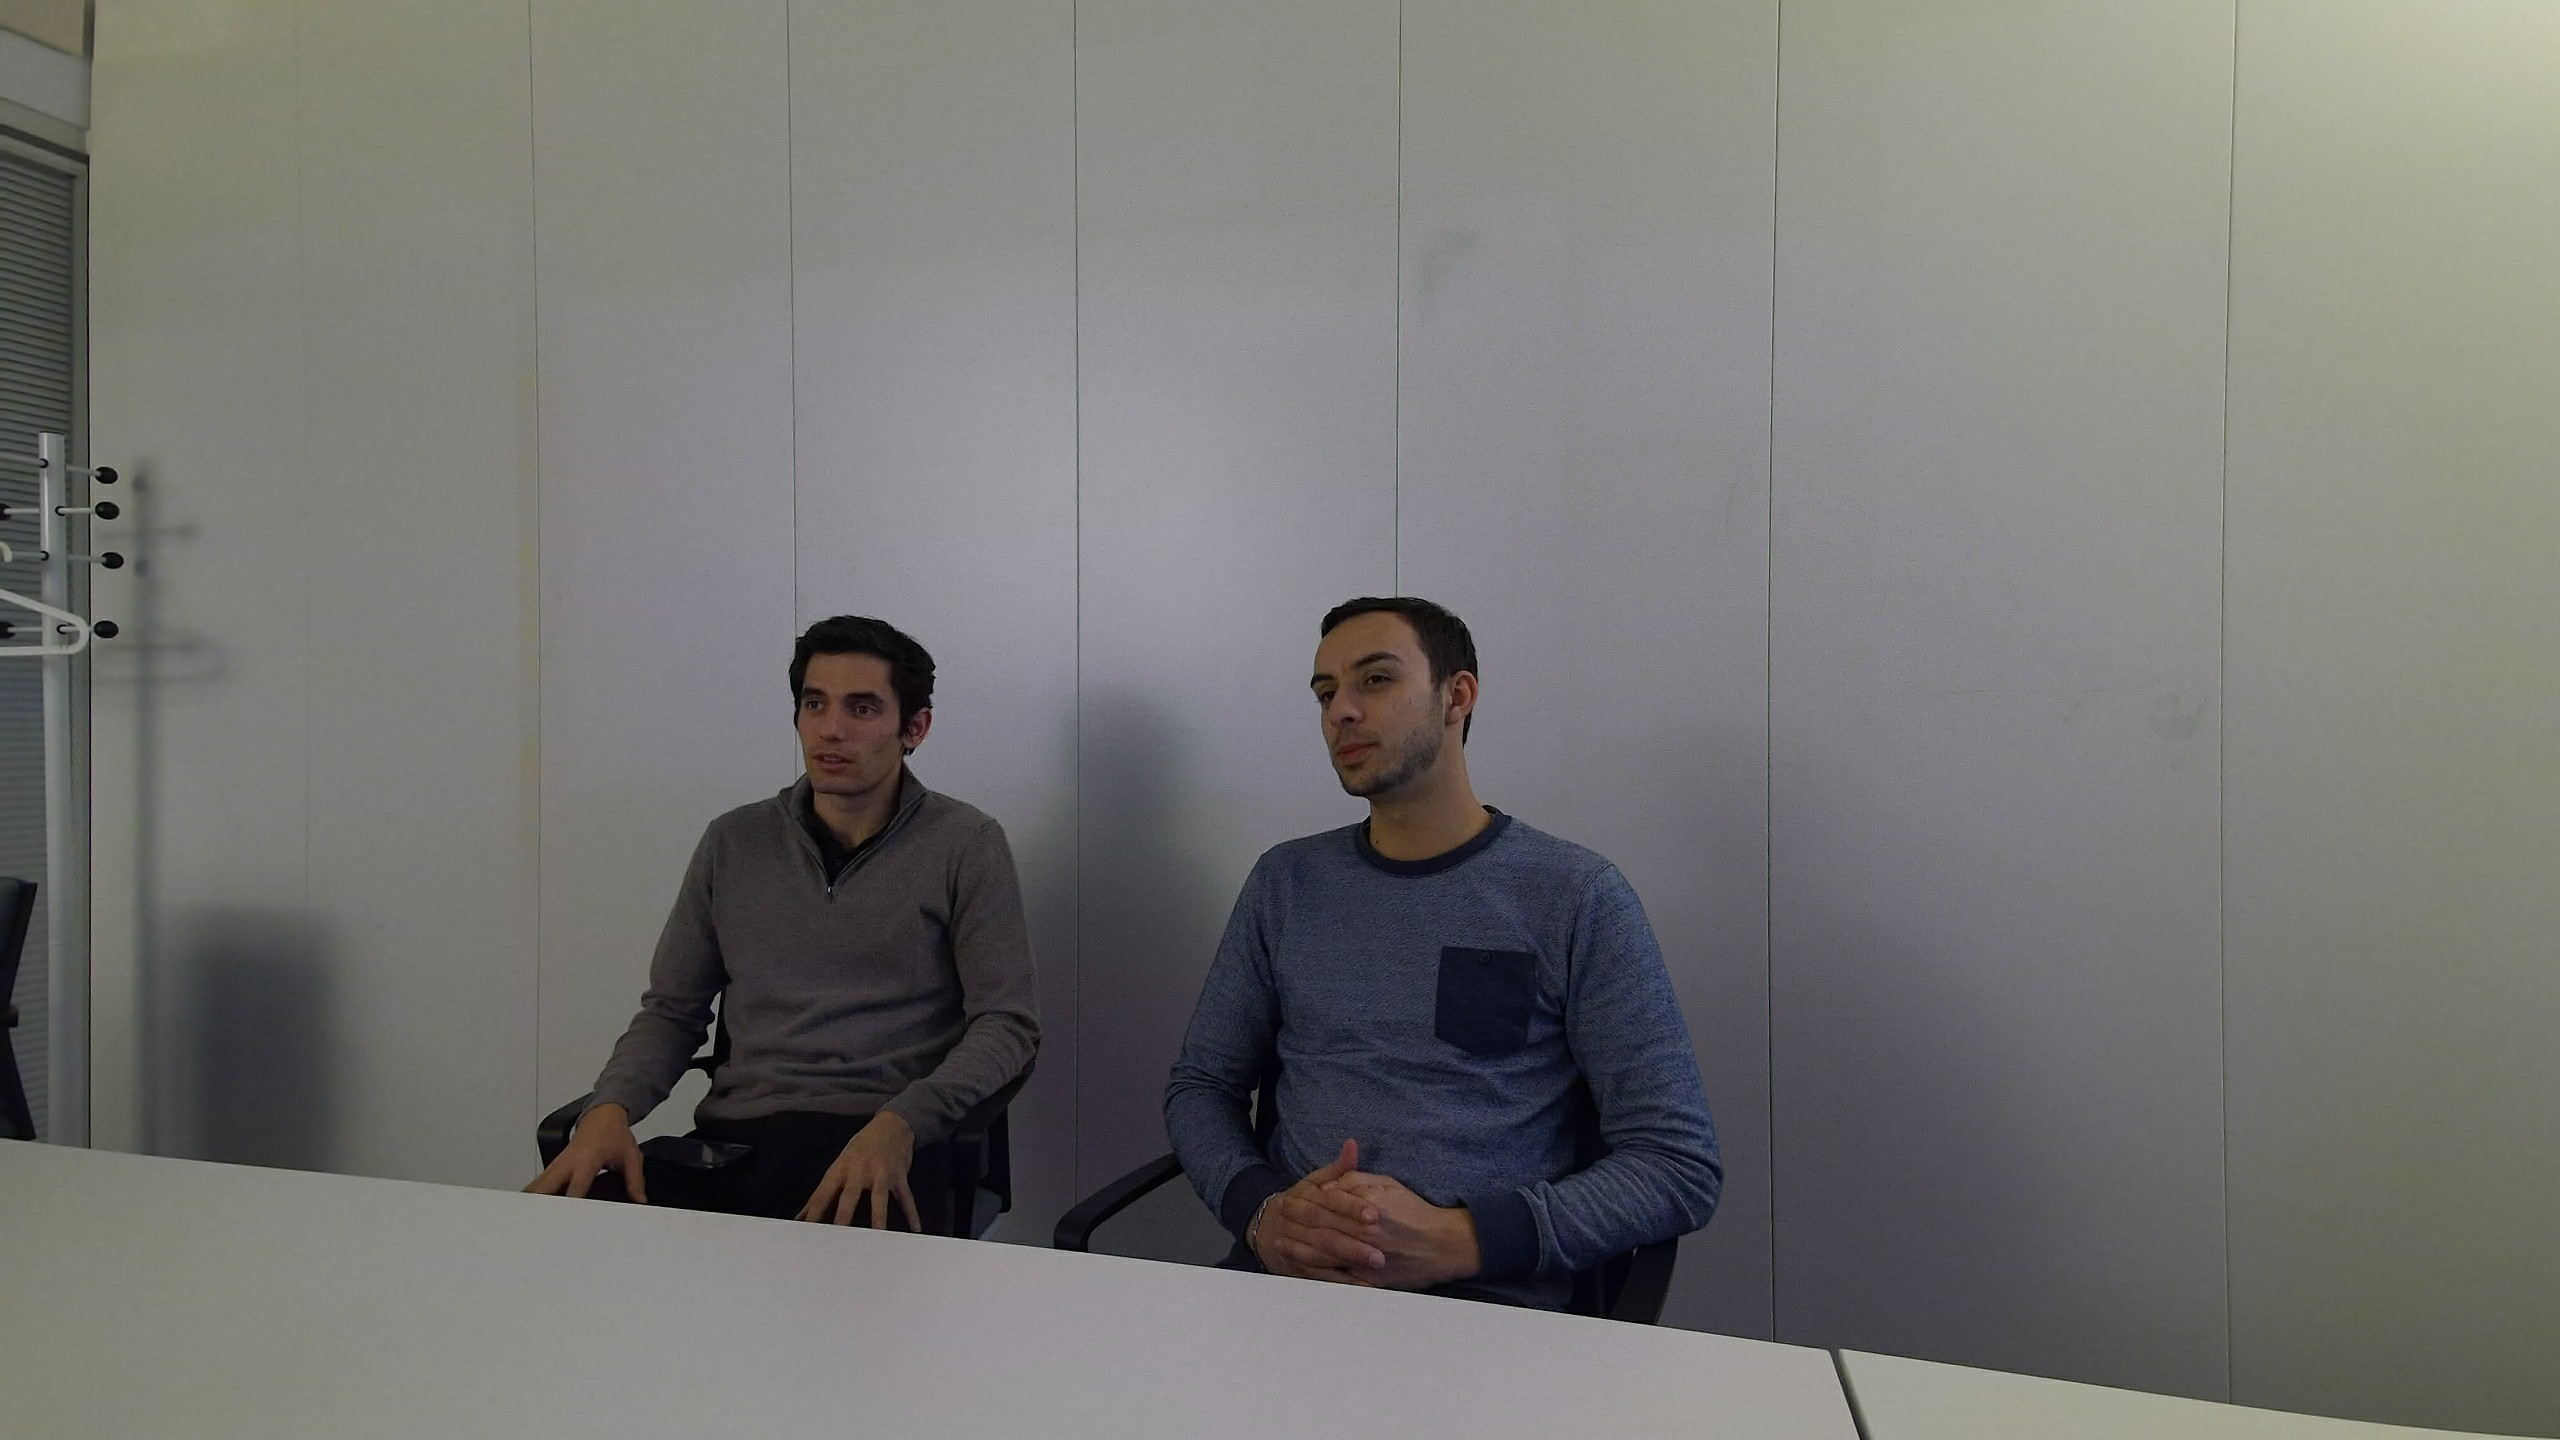
\includegraphics[width=\textwidth]{images/scenario/00790_master.jpg}
    \caption{2D original view 1}
    \label{figure:00790_master}
  \end{subfigure}
  \hfill
  \begin{subfigure}[b]{0.48 \textwidth}
    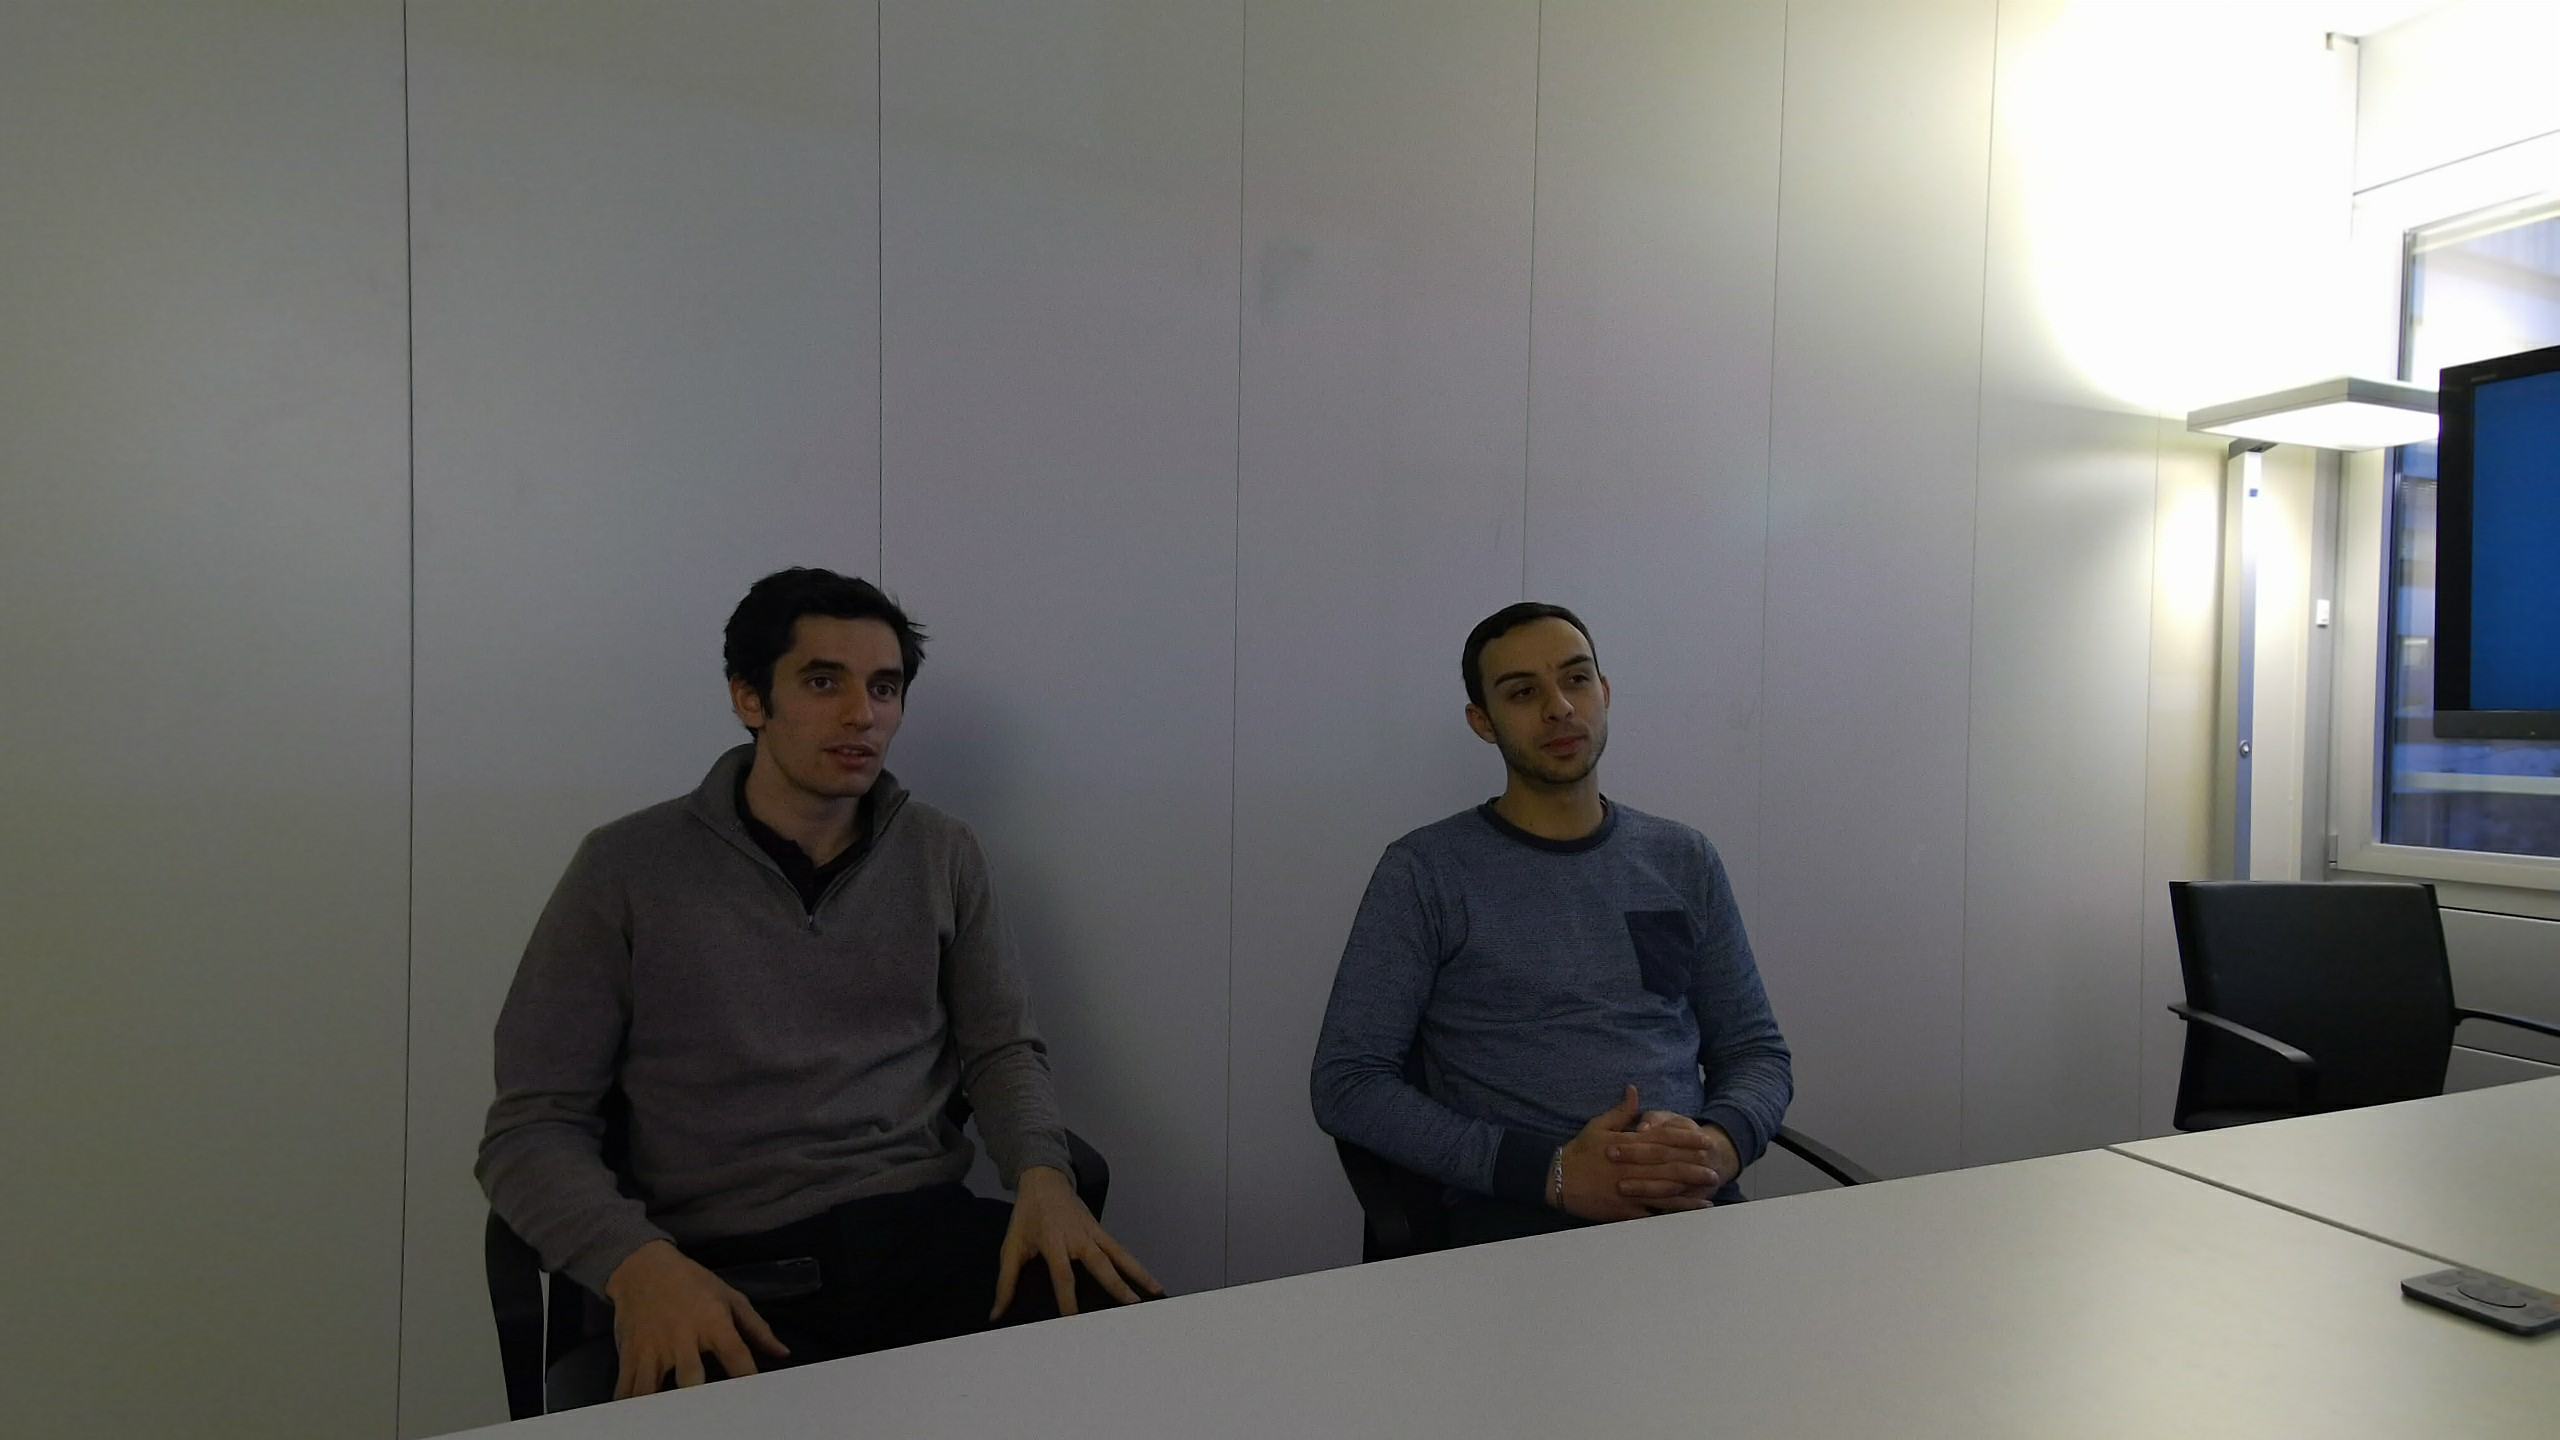
\includegraphics[width=\textwidth]{images/scenario/00790_sub.jpg}
    \caption{2D original view 2}
    \label{figure:00790_sub}
  \end{subfigure}
  \hfill
  \begin{subfigure}[b]{0.48 \textwidth}
    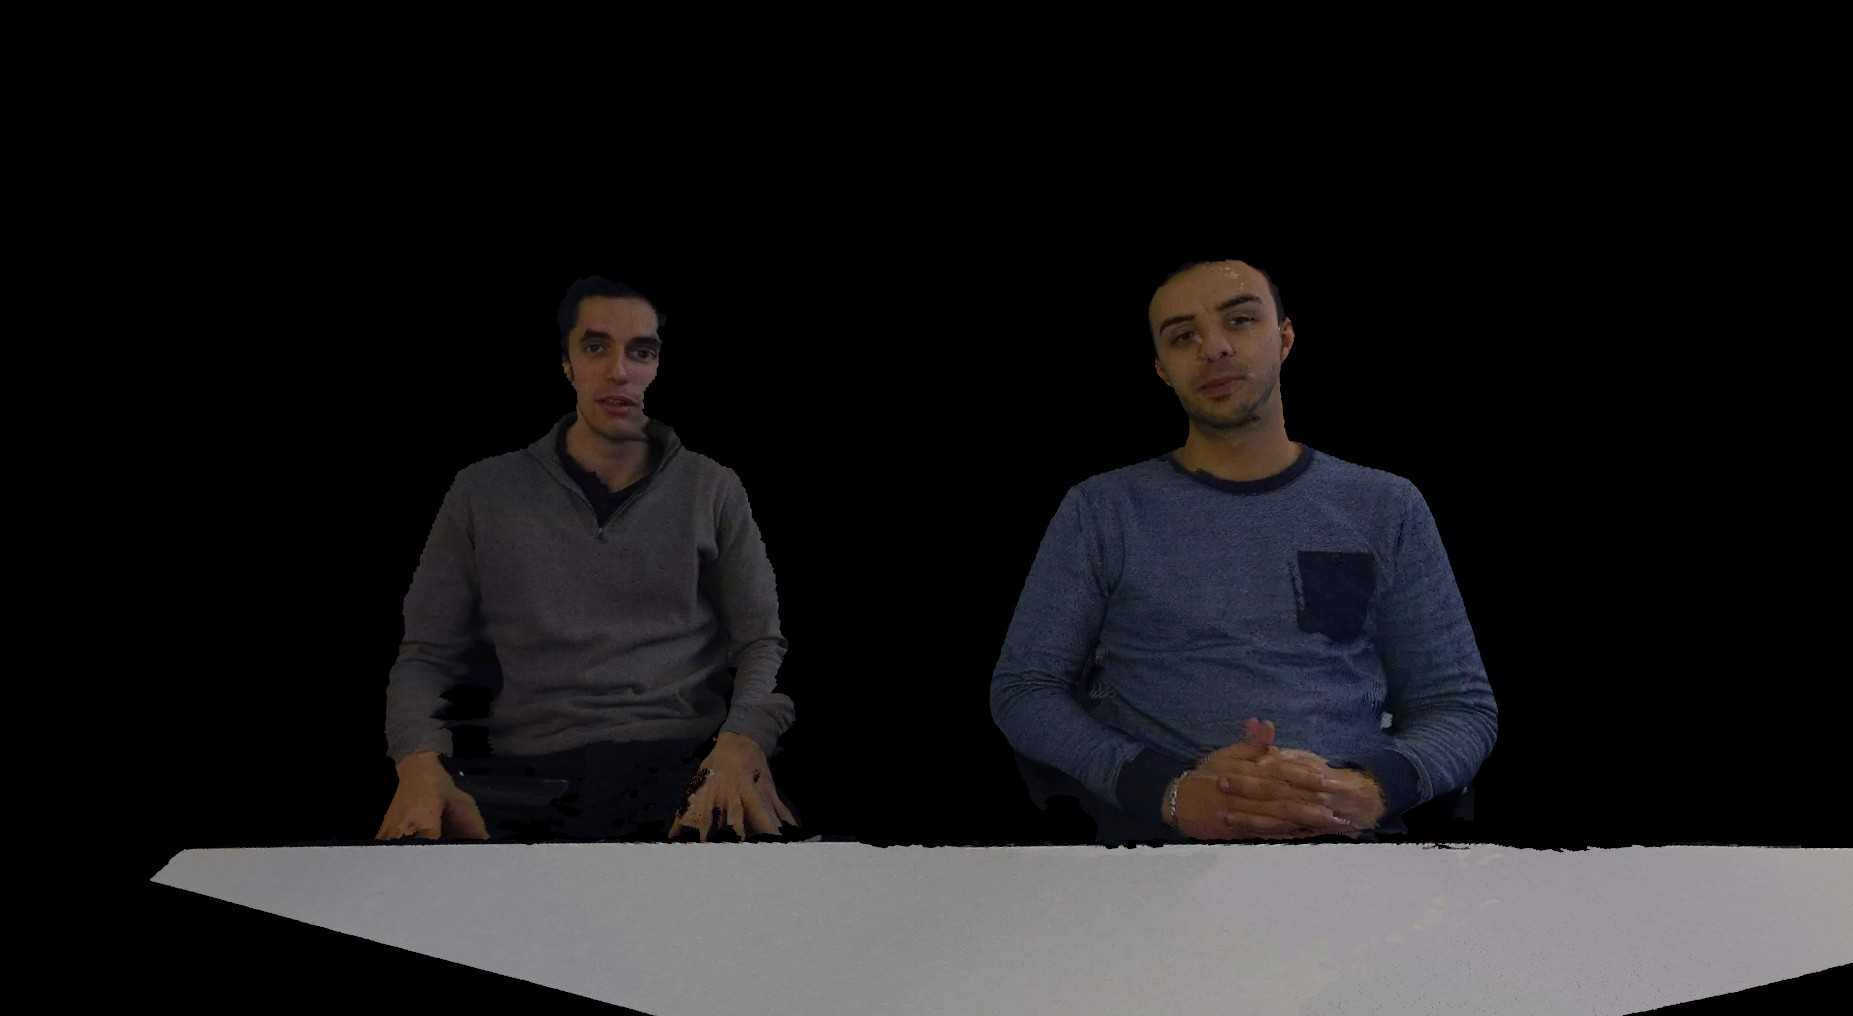
\includegraphics[width=\textwidth]{images/scenario/00790_pc_2.jpg}
    \caption{Virtual point of view without background}
    \label{figure:00790_pc_2}
  \end{subfigure}
  \hfill
  \begin{subfigure}[b]{0.48 \textwidth}
    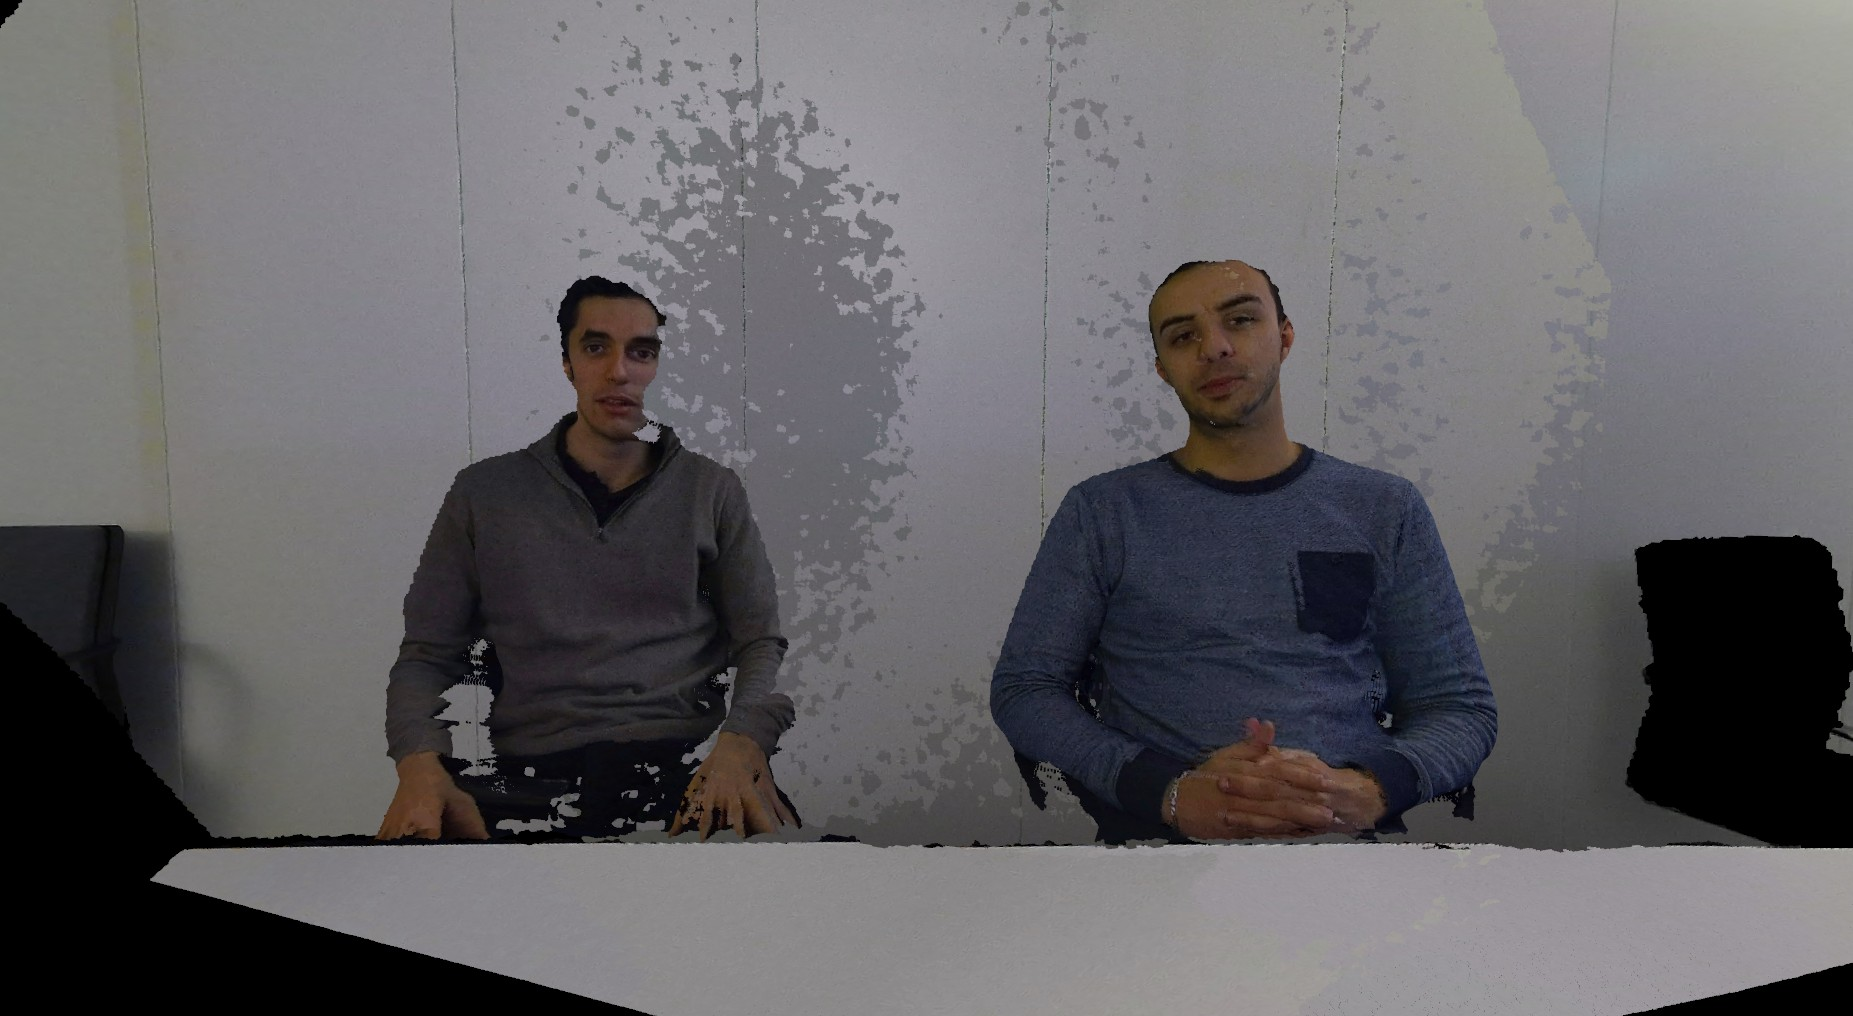
\includegraphics[width=\textwidth]{images/scenario/00790_background.jpg}
    \caption{Virtual point of view with background}
    \label{figure:00790_background}
  \end{subfigure}
  \caption{Rendering of a selected frame from 2D original views, see figure \ref{figure:00790_master} \& \ref{figure:00790_sub}. Same virtual viewpoint of the scene \ref{figure:00790_pc_2} \& \ref{figure:00790_background}}
  \label{figure:two_persons_virtualview}
\end{figure}

 
\subsection{Streaming for gamer}
 
 Streaming in video games is popular. Logitech has recently acquired \textit{Streamlabs} which is a live streaming software service. Streamers are using traditional 2D RGB cameras. Therefore, the point of view of the video stream is not always optimal and is fixed during the whole session. Using RGB-D cameras to enable viewers to change freely the point of view could improve the immersion and the quality of the streaming session. This scenario wasn't investigated in this thesis but could the subject of another project. It could be an alternative application of such this 3D technology for Logitech.

%  \section{hello2}
%  \subsection{hello3}
%  \subsubsection{hello4}
%  \subsubsubsection{hello5}